\section{Datasets  \fixme{Maybe be a chapter instead of section?}}\label{s:datasets}
As we have stated in section \ref{s:two-types-of-data}, the input data can have many different types, since our system can serve a wide variety of applications.
We have separated the data in two broad categories -- categorical and continuous, therefore our algorithms are also logically separated for those two different kinds of data.

The second reason that we separated our algorithms in those two types, was that we experimented with datasets both types.
In medical research it is common to have standard datasets with continuous exact values corresponding to a set of attributes, but it is also common for the datasets to be semantically annotated.
For instance a dataset of the first form could have a column corresponding to attribute \textit{Height (cm)} with values including $146.84, 139.35, 189.00, 182.68, 160.19, 138.66, 173.06$ etc.
On the other hand, a dataset of the second time would have normalized values including $Tall, Average, Short$ etc.
The synthetic datasets we had available for experimentation were the following.

\textbf{CVI Dataset:}
Cardiovascular disease is a class of diseases that involve the heart or blood vessels.
Cardiovascular disease includes coronary artery diseases (CAD) such as angina and myocardial infarction (commonly known as a heart attack).
This dataset contains CardioVascular Imaging (CVI) information, which are represented as numerical values – not normalized.
The format of this dataset is the standard tabular format, we find in CSV files or in tables of relational databases.
An (incomplete) example can be found in table \ref{t:cvi}.

\begin{table}[H]
  \centering
  \caption{CVI dataset}
  \label{t:cvi}
\begin{center}
  \begin{tabular}{ c | c | c | c | c}
    Heart rate & Height (cm) & Weight (kg) & LVEDV (ml) & ... \\
   \hline
   90 & 146.84 & 61.94 & 118.36 & ... \\
   82 & 139.35 & 41.51 & 133.39 & ... \\
   $\vdots$ & $\vdots$ & $\vdots$ & $\vdots$ & $\vdots$ \\
  \end{tabular}
\end{center}
\end{table}

\textbf{MeSH Dataset:}
MeSH\footnote{\href{https://meshb.nlm.nih.gov/}{https://meshb.nlm.nih.gov/}} provides a hierarchically-organized\footnote{\href{https://meshb.nlm.nih.gov/treeView}{https://meshb.nlm.nih.gov/treeView}} terminology for indexing and cataloging of biomedical information such as MEDLINE/PUBmed and other United States National Library of Medicine (NLM) databases.
Created and updated by the NLM, it is used by articles databases and by NLM's catalog of book holdings.
This dataset is based on the MeSH tree structure.
MeSH terms are represented as normalized values; this means that for instance attributes like Age, are separated into groups (for instance Child, Adult, etc).
This dataset contains semantically annotated patient data.
The layout of this dataset is quite different from the ordinary tabular data format, it follows the DATS format.
DATS is the underlying model powering metadata ingestion, indexing and searches in DataMed, a NIH (National Institute of Health - US) funded project that aims to represent for biomedical datasets what PubMed (https://www.ncbi.nlm.nih.gov/pubmed) is for the biomedical literature.
The DATS model is designed around the \textit{Dataset} element as shown in figure \ref{f:dats}.



\begin{figure}[H]
  \centering
  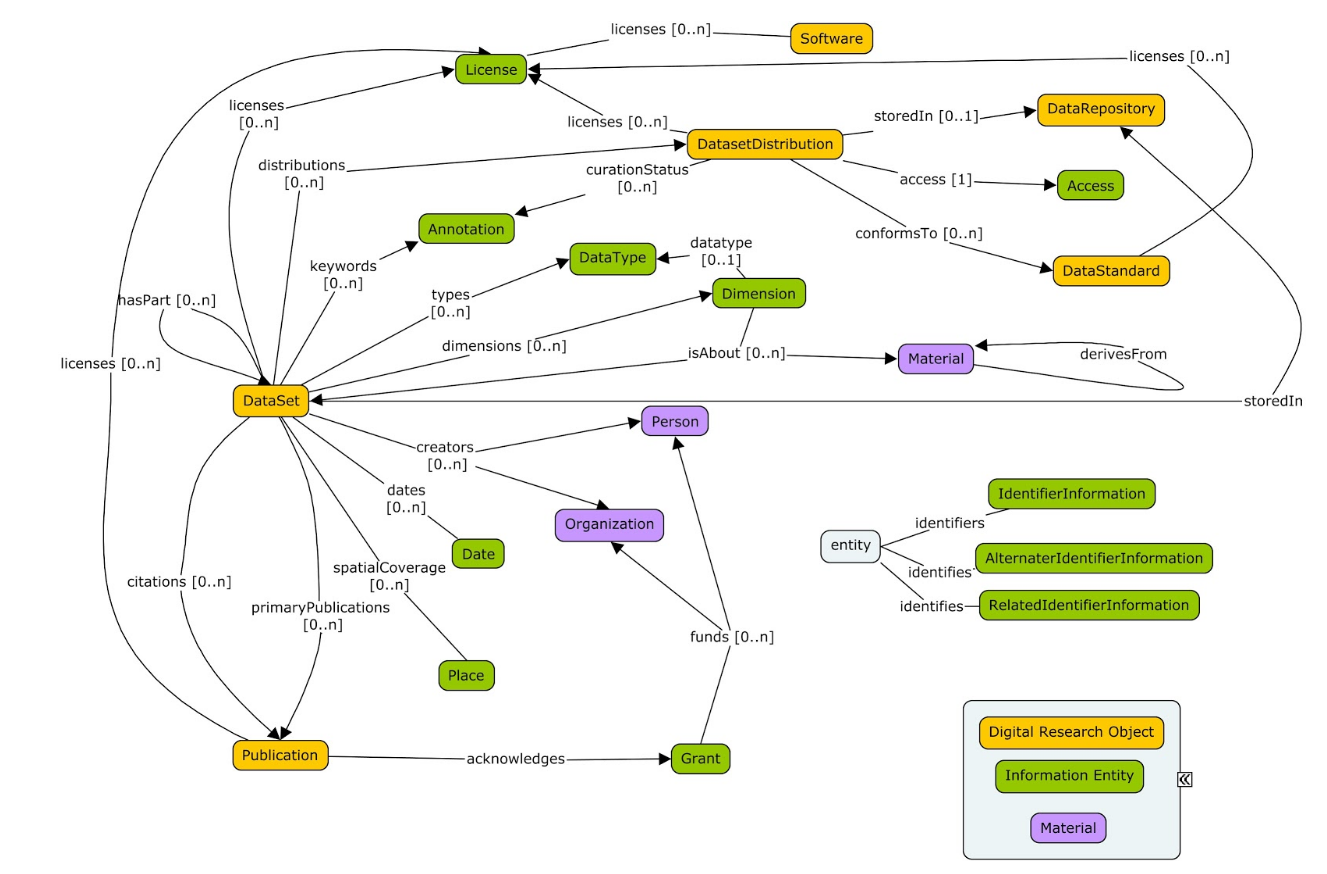
\includegraphics[width=\columnwidth]{figures/dats.png}
  \captionof{figure}{DATS model}
  \label{f:dats}
\end{figure}

Among other metadata, the DATS model contains the \textit{keywords} element which is a set consisting of (in our case) MeSH codes.
As a result, our dataset is comprised of a JSON object for each patient.
This JSON object contains a \textit{keywords} element with a list of MeSH codes describing that patient.
An example can be seen in Code \ref{sc:mesh-json}.


{
\begin{minted}[framesep=3mm, frame=single, tabsize=2, breaklines, breaksymbolleft=, fontsize=\footnotesize]{json}
  {
      "keywords": [
          {
              "value": "Women",
              "valueIRI": "https://meshb.nlm.nih.gov/record/ui?ui=D014930"
          },
          {
              "value": "Adult",
              "valueIRI": "https://meshb.nlm.nih.gov/record/ui?ui=D000328"
          },
          {
              "value": "African Americans",
              "valueIRI": "https://meshb.nlm.nih.gov/record/ui?ui=D001741"
          },
          .
          .
          .
      ],
      .
      .
      .
  }
\end{minted}
\captionof{lstlisting}{Example of a patient JSON object with MeSH codes}
\label{sc:mesh-json}
}

The problem with this approach is that the information about a patient is ``flat'' as it does not follow the \textit{attribute\hyp value} model, it is just a set of MeSH terms.
In order to import it in our private secret\hyp shared database that resides in the SMPC cluster, we need to transform this kind of data to a tabular structure.
For that reason we developed a procedure that performs this conversion at the time of secure importing.
This procedure considers the importing attributes as the ``column'', and its direct (1 level down) child that is a parent of the found keyword as the ``value''.

To demonstrate how this conversion works, considered the following (incomplete) hierarchy of MeSH terms.
\dirtree{%
.1 Anatomy [A].
.1 Organisms [B].
.1 Diseases [C].
.2 Bacterial Infections and Mycoses [C01].
.2 Virus Diseases [C02].
.2 Parasitic Diseases [C03].
.2 Neoplasms [C04].
.2 Musculoskeletal Diseases [C05].
.2 Digestive System Diseases [C06].
.2 Stomatognathic Diseases [C07].
.3 Ankyloglossia [C07.160].
.3 Jaw Diseases [C07.320].
.3 Mouth Diseases [C07.465].
.3 Pharyngeal Diseases [C07.550].
.3 Stomatognathic System Abnormalities [C07.650].
.3 Temporomandibular Joint Disorders [C07.678].
.4 Temporomandibular Joint Dysfunction Syndrome [C07.678.949].
.3 Tooth Diseases [C07.793] .
.2 ....
.1 ....
}

Lets also assume that the JSON object of a patient contains the keyword \textit{Temporomandibular Joint Dysfunction Syndrome [C07.678.949]} and that the chosen attribute for importing is \textit{Diseases [C]}.
In this case we will take \textit{Diseases [C]} as the ``column'' and \textit{Stomatognathic Diseases [C07]} as the ``value'', since it is the direct ``child'' of the chosen attribute, which is a ``parent'' of \textit{Temporomandibular Joint Dysfunction Syndrome [C07.678.949]} found in the patient JSON object. The resulting (partial) table can be seen in table \ref{t:json-to-csv-1}.
If the chosen attribute for importing was \textit{Stomatognathic Diseases [C07]} instead of \textit{Diseases [C]}, then the ``column'' would be \textit{Stomatognathic Diseases [C07]}, and the ``value'' would be \textit{Temporomandibular Joint Disorders [C07.678]}. The resulting (partial) table can be seen in table \ref{t:json-to-csv-2}.

\begin{minipage}{0.45\textwidth}
  \begin{table}[H]
    \centering
    \caption{Importing of Diseases [C]}
    \label{t:json-to-csv-1}
  \begin{center}
    \begin{tabular}{ c | c}
     Diseases & ... \\
     \hline
     Stomatognathic Diseases & ... \\
     $\vdots$ & $\vdots$ \\
    \end{tabular}
  \end{center}
\end{table}
\end{minipage}
\begin{minipage}{0.45\textwidth}
  \begin{table}[H]
    \centering
    \caption{Importing of Stomatognathic Diseases [C07]}
    \label{t:json-to-csv-2}
  \begin{center}
    \begin{tabular}{ c | c}
     Stomatognathic Diseases & ... \\
     \hline
     Temporomandibular Joint Disorders & ... \\
     $\vdots$ & $\vdots$ \\
    \end{tabular}
  \end{center}
\end{table}
\end{minipage}


